\section{Interferometry and the Inverse Problem}\label{intro}
Astronomy requires its instruments to have a high angular resolutions. This is an issue for radio wavelengths: The longer the wavelength, the bigger the diameter of a single dish antenna. Single dish antenna's are expensive to build and harder to steer accurately. Interferometers, where multiple smaller antennas act as a single large instrument, have had great success in Radio Astronomy. Instruments like VLA, ALMA and LOFAR have produced high-resolution images. 

Interferometers do not observe the sky directly. Each antenna pair measure Fourier Components (Visibilities) of the sky brightness. The observed image has to be reconstructed from the measured Visibilites. Since the interferometer can only observe a limited number of Visibilities, the reconstruction is an ill-posed inverse problem.

For small Field of View imaging, the CLEAN class of Algorithms\cite{many} have been developed and is the de-facto standard in Radio Astronomy. It is not guaranteed to reconstruct the true image in theory, it has produced remarkable results with expert tuning. New generation Interferometers like ASKAP, Pathfinder and SKA are built with wide Field of View imaging in mind. The CLEAN Algorithms have been extended for Wide Field of Views, but require even more tuning by experts. 

The Theory of Compressed Sensing\cite{many} has seen success in solving ill-posed inverse problems in other fields like image de-noising\cite{many}, in-painting\cite{many} and super-resolution\cite{many}. Applying the Theory of Compressed Sensing to Radio Interferometry is an active field of research. 

It can work in Wide Field imaging, It has the potential to reduce the expert tuning, is guaranteed to reproduce the true image under the right conditions and has the potential to super-resolve.

A proof of concept Compressed Sensing Algorithm implemented in the Common Astronomy Software Application (CASA).

\subsection{Inverse Problem for small Field of View Imaging}
For small Field of Views, the inverse problem can be simplified(although it is still ill-posed). Each antenna pair measures a Visibility of the sky brightness. The distance between the antenna's 


For the current class of interferometers, retrieving the observed image of the sky is calculating the Inverse Fourier Transform of the measured Visibilities. (This is a simplification of the actual problem, which does not hold true for future instruments like SKA. How the Inverse Problem changes for future instruments is handled in section \ref{radio}). Since the Visibility Space is undersampled, the resulting image is 'dirty', as it contains effects from the instrument. The effects of the instrument can be modelled as a Point Spread Function (PSF). The Dirty Image is the Result of the True Image convolved with the PSF. Figure \ref{intro:inverse_problem} shows an example of the PSF, Dirty Image and True Image.
\begin{figure}[h!]
	\centering
	\begin{subfigure}[b]{0.3\linewidth}
		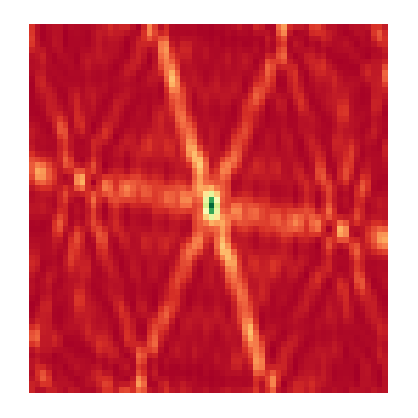
\includegraphics[width=\linewidth, trim={18px 19px 18px 18px}, clip]{./chapters/01.intro/img/psf.png}
		\caption{Point Spread Function (PSF)}
	\end{subfigure}
	\begin{subfigure}[b]{0.3\linewidth}
		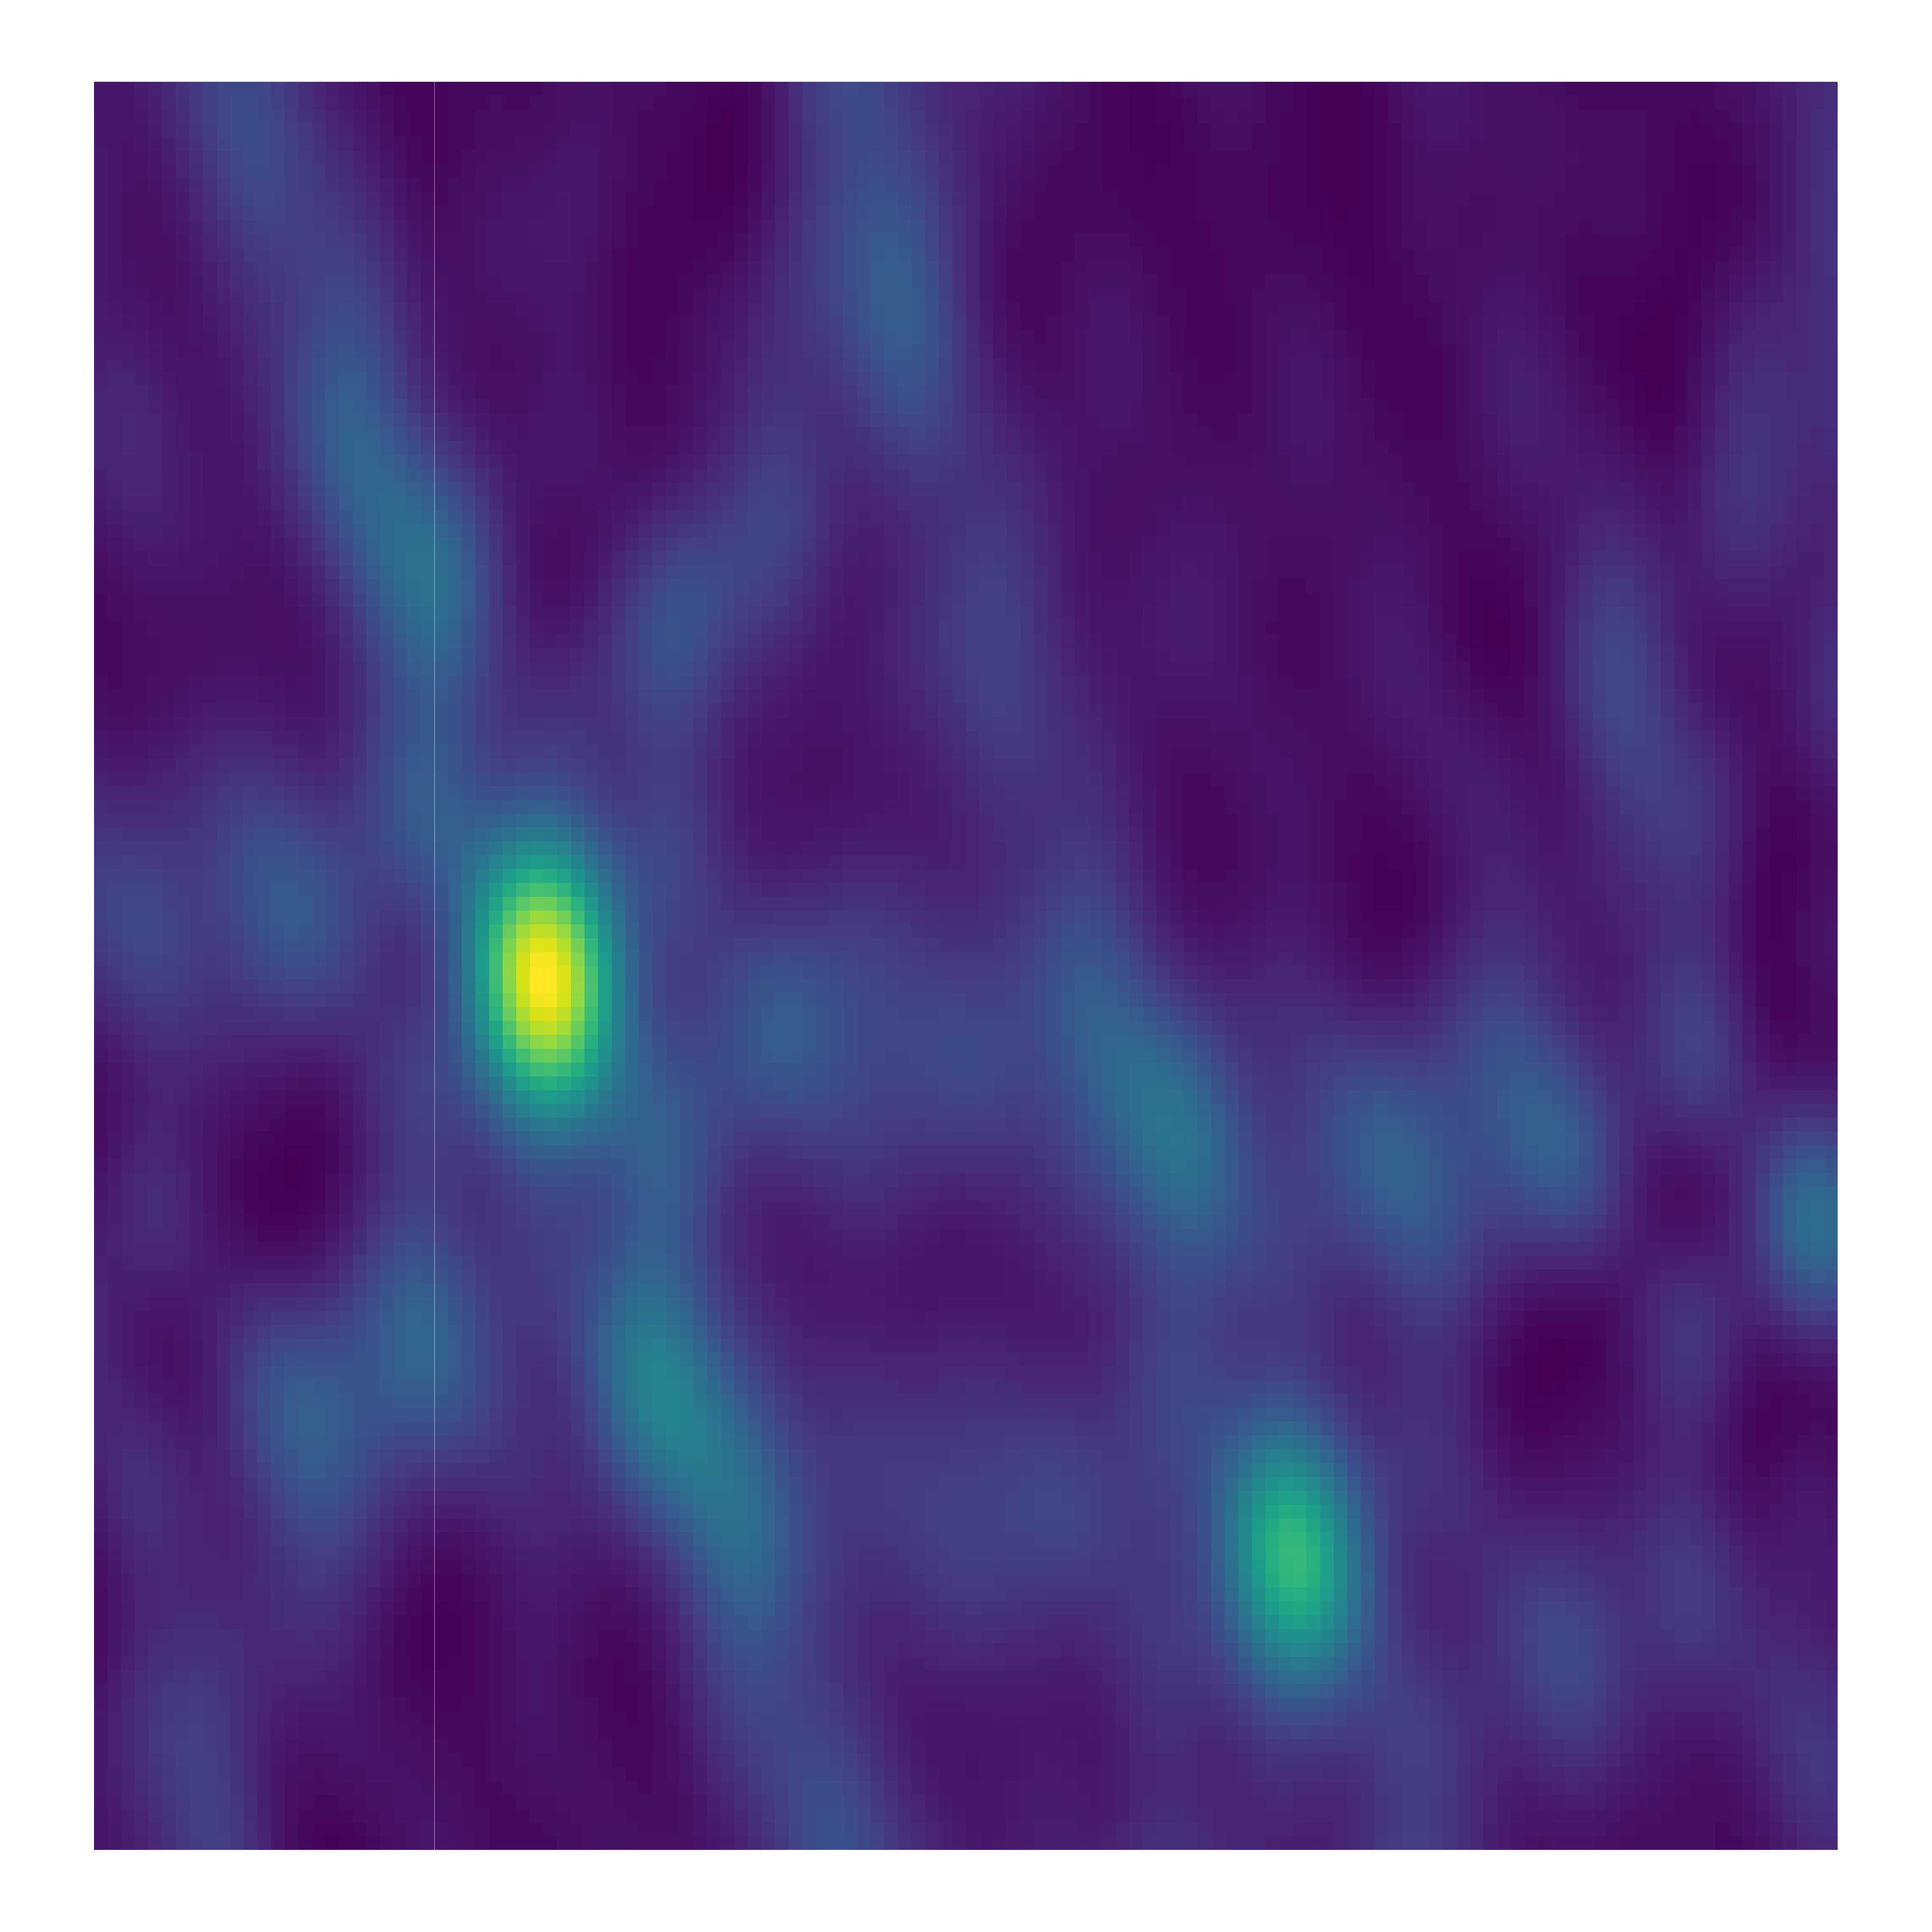
\includegraphics[width=\linewidth, trim={18px 19px 18px 18px}, clip]{./chapters/01.intro/img/dirty_image.png}
		\caption{Dirty Image}
	\end{subfigure}
	\begin{subfigure}[b]{0.3\linewidth}
		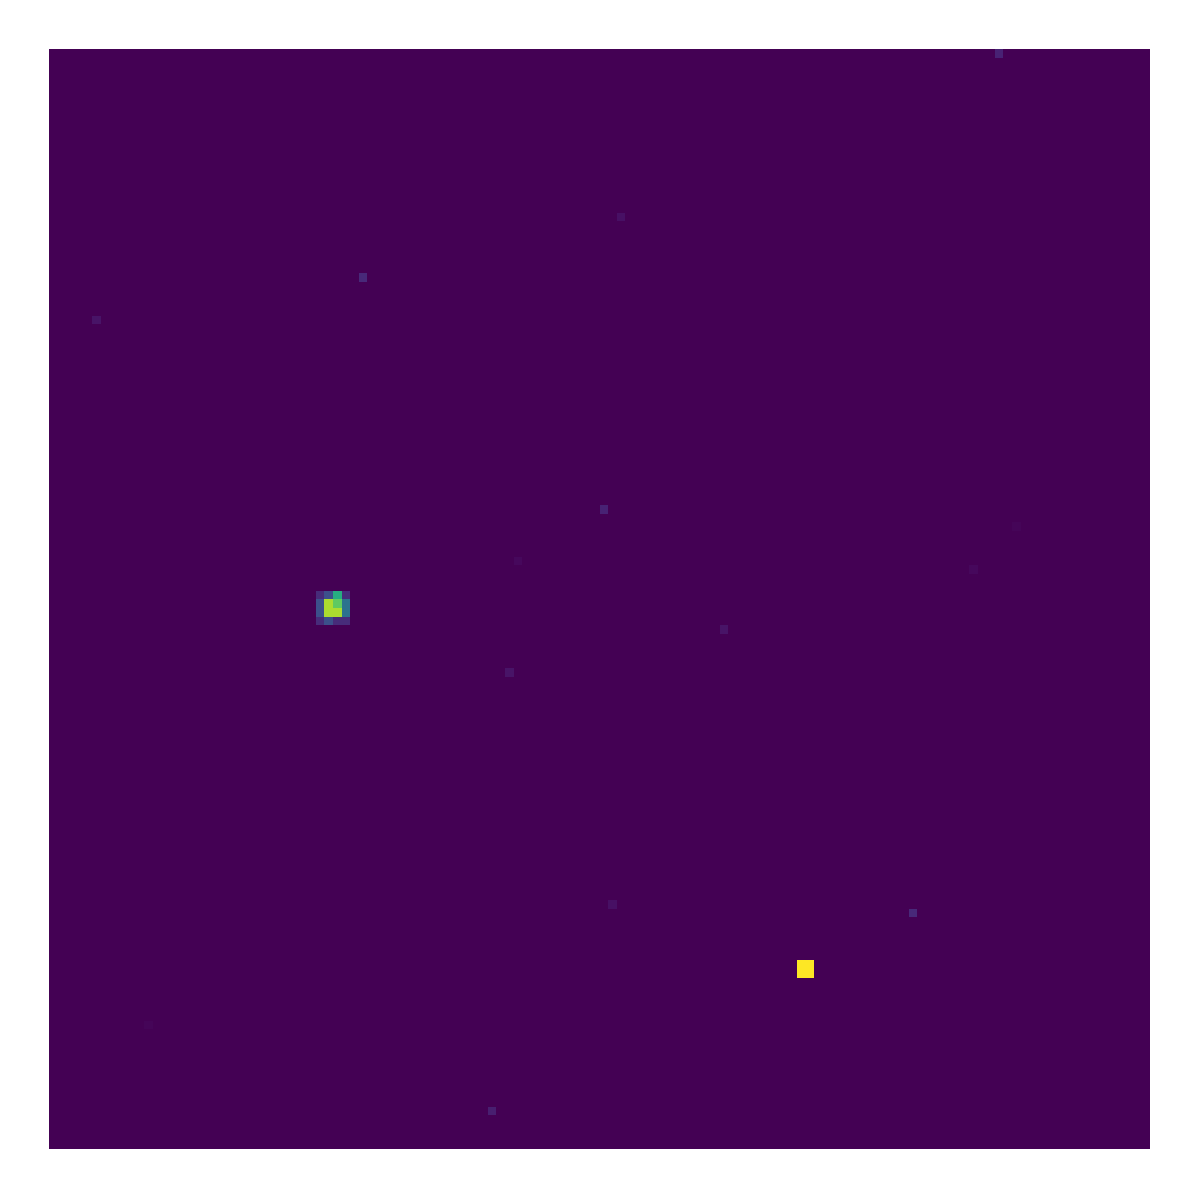
\includegraphics[width=\linewidth, trim={18px 19px 18px 18px}, clip]{./chapters/01.intro/img/true_image.png}
		\caption{True Image}
	\end{subfigure}
	\caption{The Inverse Problem: Finding the true image of the sky when only the PSF and the dirty image are known.}
	\label{intro:inverse_problem}
\end{figure}

The Dirty Image is the result of the Inverse Fourier Transform, the PSF on the other hand follows directly from the antenna configuration. Figure \ref{intro:ANT_UV_PSF} shows an example of the VLA instrument. 

Inverse Fourier Transform

\begin{figure}[h!]
	\centering
	\begin{subfigure}[b]{0.3\linewidth}
		 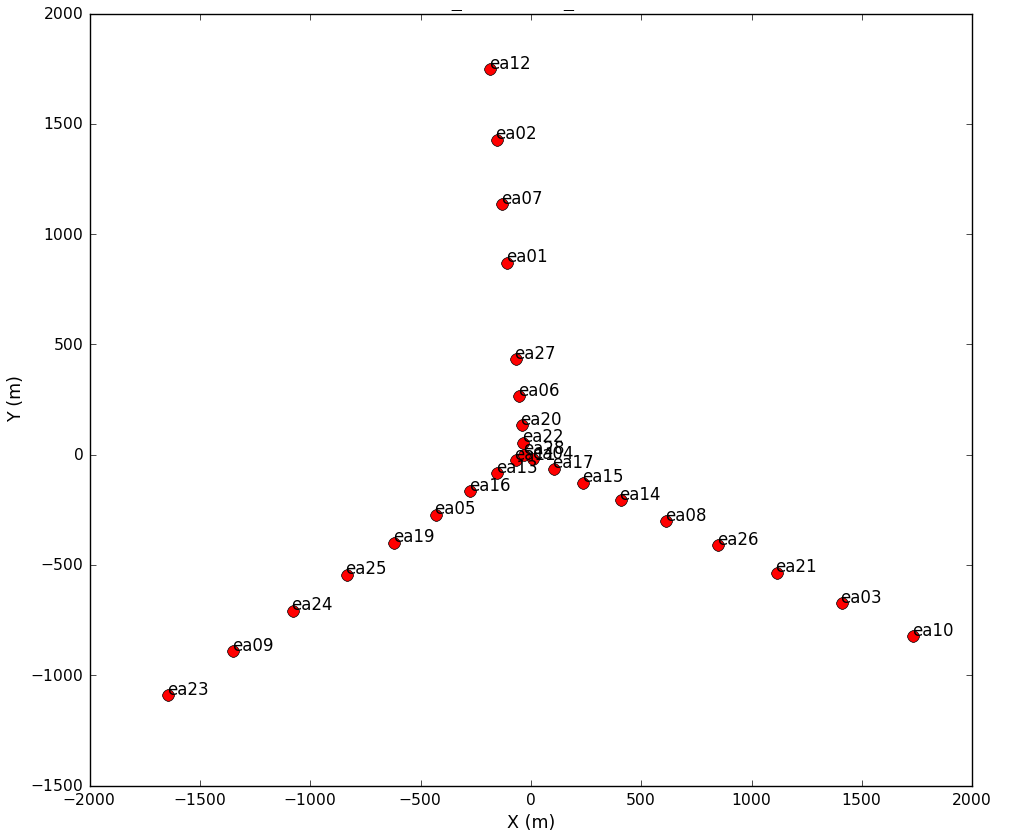
\includegraphics[width=\linewidth, trim={18px 19px 18px 18px}, clip]{./chapters/01.intro/img/antennas.png}
		 \caption{Antenna Configuration}
	\end{subfigure}
	\begin{subfigure}[b]{0.3\linewidth}
		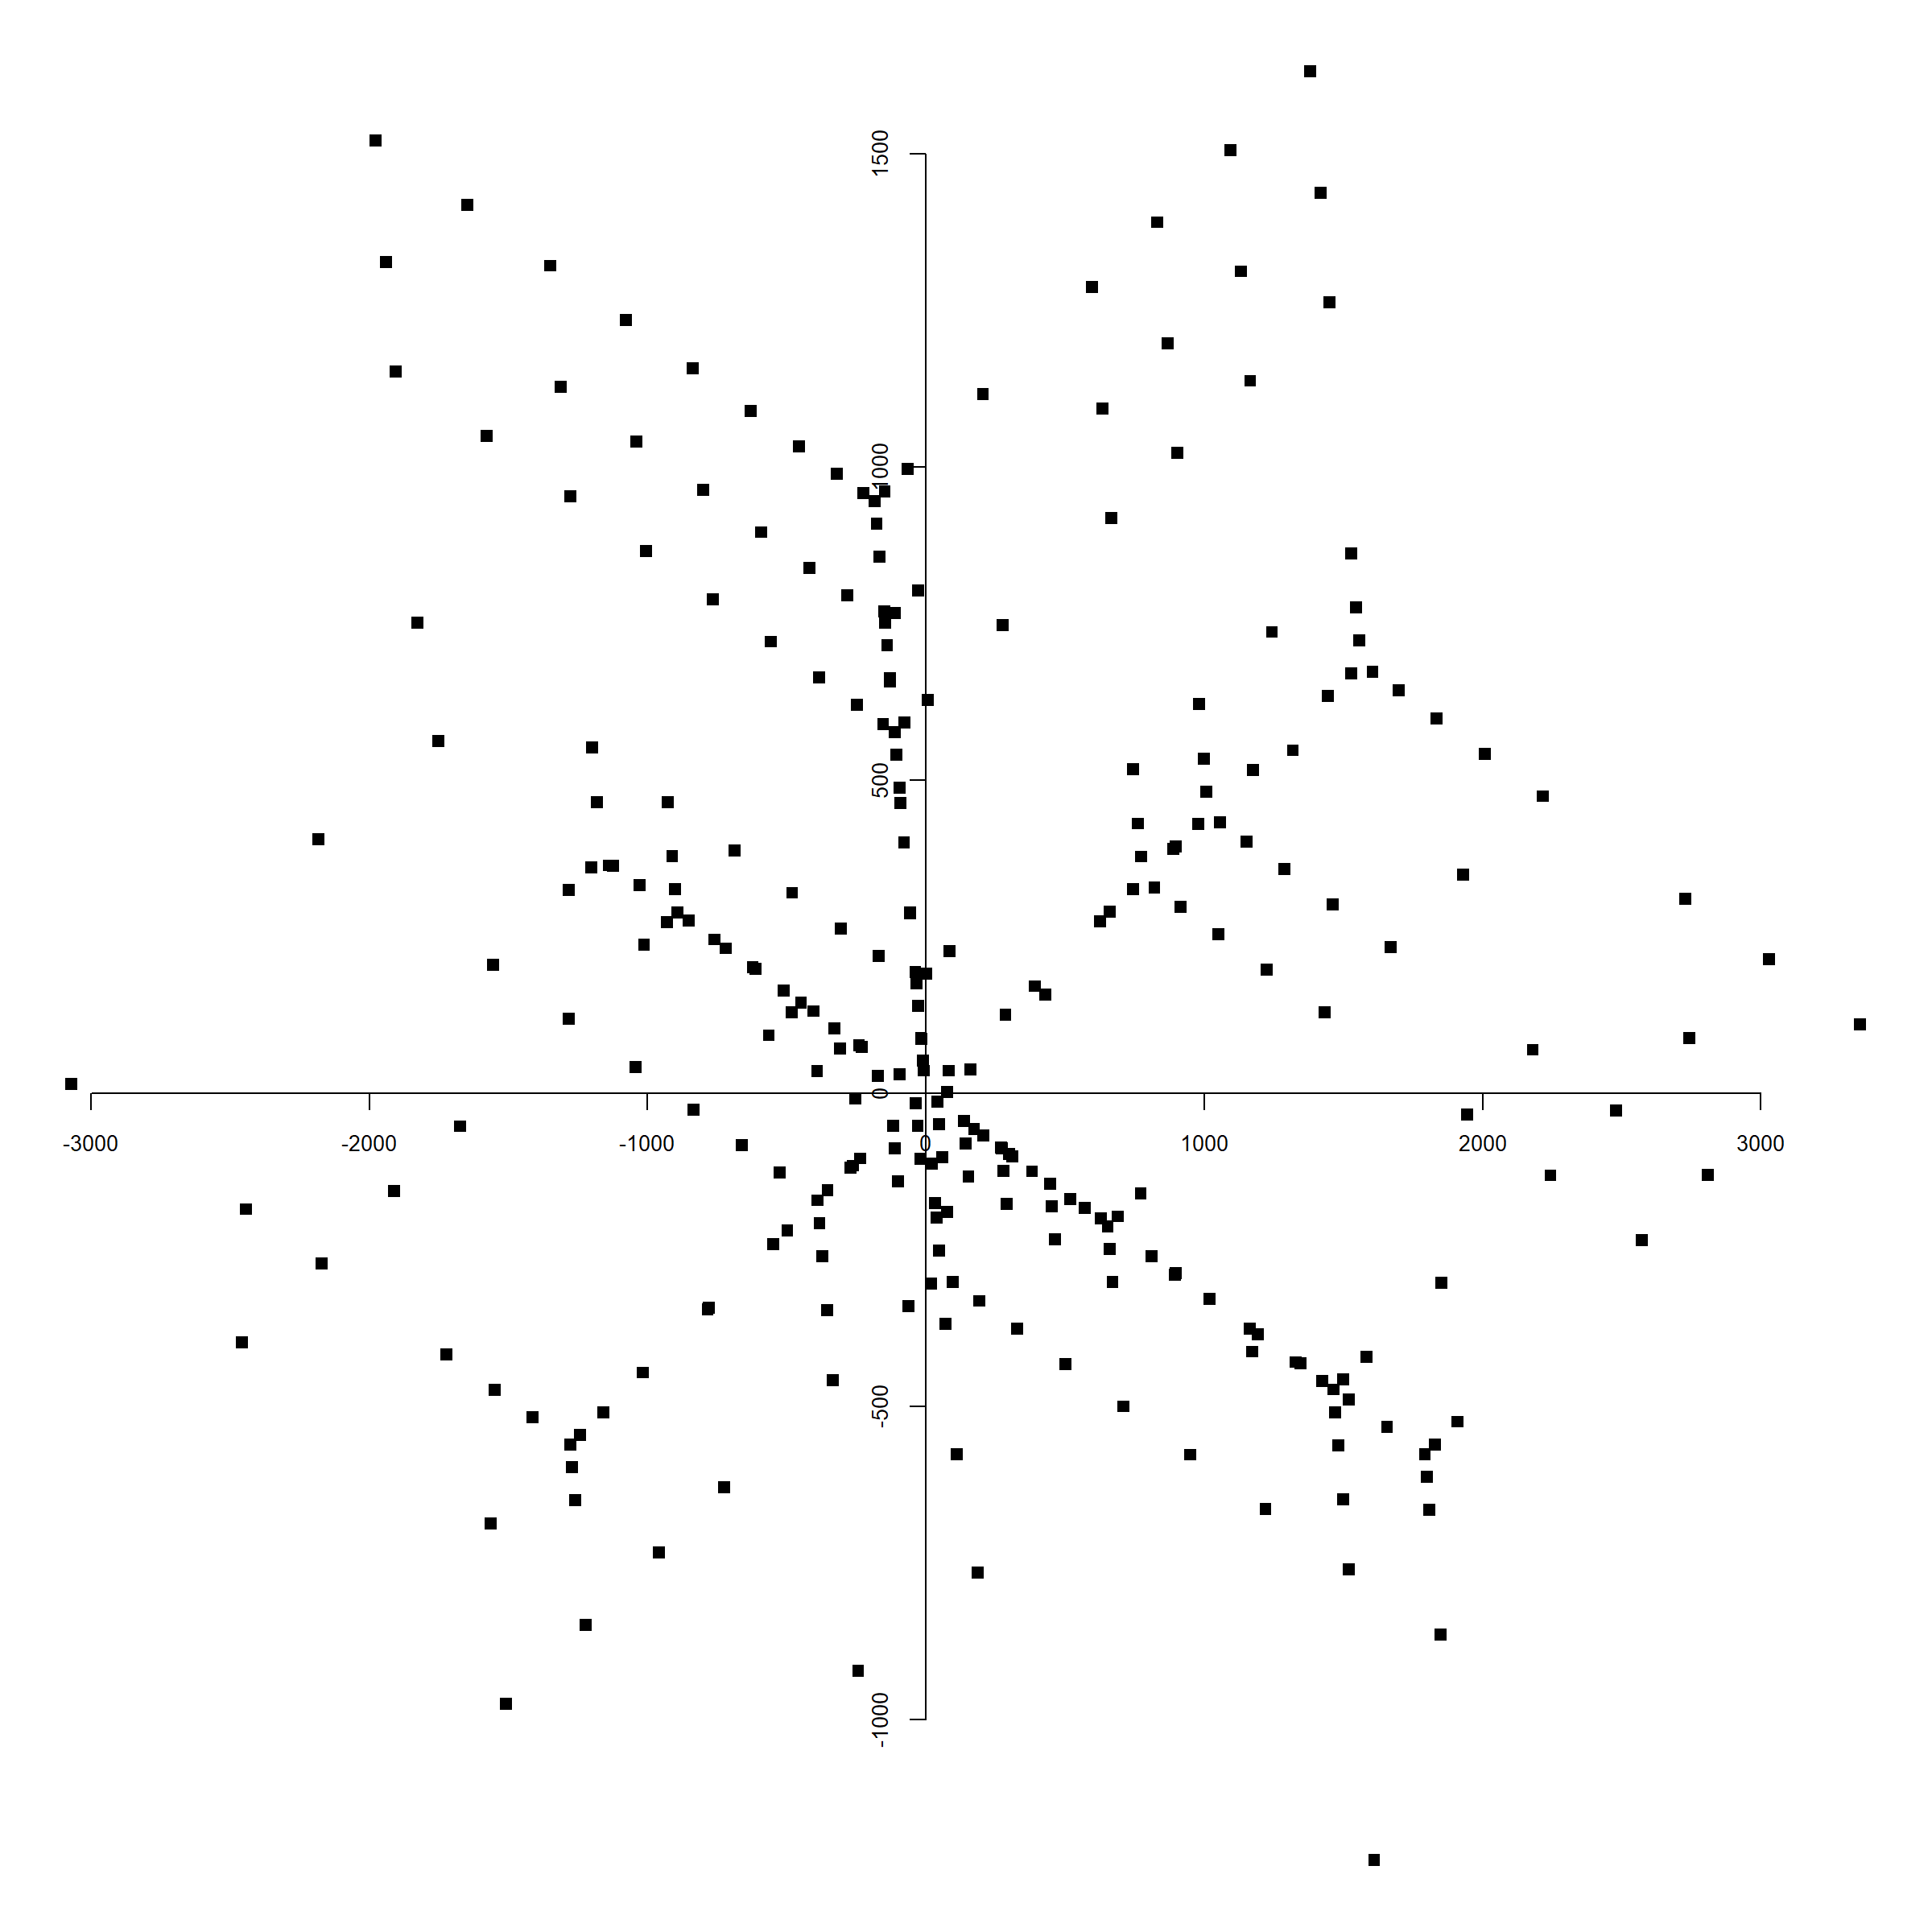
\includegraphics[width=\linewidth, trim={18px 19px 18px 18px}, clip]{./chapters/01.intro/img/uv.png}
		\caption{UV Space}
	\end{subfigure}
	\begin{subfigure}[b]{0.3\linewidth}
		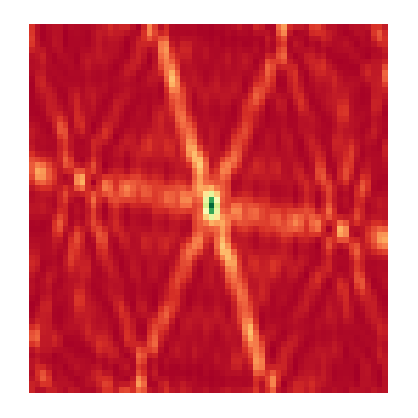
\includegraphics[width=\linewidth, trim={18px 19px 18px 18px}, clip]{./chapters/01.intro/img/psf.png}
		\caption{Point Spread Function (PSF)}
	\end{subfigure}
	\caption{The Antenna Configuration sets up the UV Space. The UV Space dictates the PSF.}
	\label{intro:ANT_UV_PSF}
\end{figure}

Each antenna pair samples a point in the UV Space. The distance between the antenna pair is called the baseline. Shorter baselines sample UV-Points closer to the center, while longer baselines sample points further away.  Each point in the UV Space represents a frequency Visibilities of the observed image: High frequency components are located away from the center and low frequency components are towards the center. Since each antenna pair contributes a Visibility, an Interferometer of $N$ antennas measures $(N-1)/2$ Visibilities. The configuration of the antenna sets up which points are sampled in the UV Space. The PSF can be calculated by using the Inverse Fourier Transform on the UV-Space. (Rotation of Earth)

Since the Dirty Image and the PSF are known, one needs to deconvolve the Dirty Image with the PSF and try to retrieve the True Image. More formally, it tries to find $X$ from the equation \eqref{intro:eq:deconvolve} in a noiseless environment.

\begin{equation}\label{intro:eq:deconvolve}
X \star  PSF = D_{dirty} 
\end{equation}

Ill-Posed

\subsection{Deconvolution with CLEAN}
The CLEAN class of Algorithms\cite{hogbom1974aperture}\cite{schwab1984relaxing}\cite{rich2008multi}\cite{rau2011multi} are widely used in Radio Astronomy. It does not solve the deconvolution problem \eqref{intro:eq:deconvolve} directly. Instead, it minimizes a similar optimization problem with the objective  \eqref{intro:eq:clean}. In each iteration, CLEAN searches the highest peak in $D_{dirty}$ and removes a fraction of the PSF at that point. It is a greedy optimizes the objective \eqref{intro:eq:clean}. It is easy to show that if CLEAN minimizes the objective to zero, then it has found a solution to the original problem \eqref{intro:eq:deconvolve}. 

\begin{equation}\label{intro:eq:clean}
\underset{X}{minimize} \: \left \| D_{dirty} - X \star PSF \right \|_2^2
\end{equation}

In a noiseless environment, the true image would be located where the objective of \eqref{intro:eq:clean} is zero. In the real world however, noise corrupts the problem and the true image may not be at the minimum any more. To address this, CLEAN is stopped early by limiting the number of iterations or when the peak is below a threshold. The algorithm should find the minimum of the objective \eqref{intro:eq:clean} where only a limited number of pixels are allowed to be non-zero; an implicit regularization term. With the right parameters, the regularization should stop the noise from corrupting the result and CLEAN should reproduce the true image.

So does CLEAN reproduce the image? It can, but it does not have to. The algorithm has no guarantees, we do not even know if the result is close to the true image. 


\subsection{From CLEAN to Compressed Sensing}
An Algorithm in the Compressed Sensing Framework has three components:
\begin{itemize}
	\item An objective function with a data and regularization term
	\item A Matrix $P$ in which the signal can be sparsely represented.
	\item An optimization algorithm that is able to handle the objective function
\end{itemize}

CLEAN can be converted into the Compressed Sensing Framework. First, the regularization term has to be explicit, it gets added to the objective function. The resulting objective \eqref{intro:eq:csclean} has two terms: A data term and a regularization term. The data term forces the reconstruction to be close to the measurement, while the regularization term forces the reconstruction to be plausible. $\lambda$ models the trade off between the terms. Note that the zero norm $\left \| PX \right \|_0$ acts as an indicator function and is not technically a norm.

\begin{equation}\label{intro:eq:csclean}
\underset{X}{minimize} \: \left \| D_{dirty} -X \star PSF \right \|_2^2 \: + \: \lambda \left \| PX \right \|_0
\end{equation}

 the new objective is the Compressed Sensing version of CLEAN. It assumes that the reconstruction is sparse in the image domain. When $P$ is the identity matrix, This is true when there are only a few point sources located in the image. Extended sources are are not well represented and are harder to detect. 
 
 The objective function is optimized by a greedy solver. 

in the compressed Sensing Framework CLEAN is
a specific objective function
with an identity matrix as prior
and a specific optimization algorithm

In this part, mostly the prior is 

The important questions are: In an undersampled, noisy environment, does the new objective \eqref{intro:eq:csclean} have a global minimum? What is the chances that the minimum is equal to the true image? It turns out that even though we have fewer samples than the Nyquist-Shannon Theorem requires, we can guarantee a global minimum and that the minimum is equal to the true image, if we have enough prior knowledge $P$ about the signal. How we model the signal and by extend, what $P$ we choose is essential for Compressed Sensing

Incoherence

\subsubsection{Modelling Prior Knowledge and Compressible Signals}


